\section{\label{appendix:mcts}MCTS Algorithm}

The following is the detailed implementation of our MCTS procedure. In each iteration of the Monte Carlo Tree Search, we start at the root, keep selecting nodes unless we find that we have selected a node never seen before, expand it, and propagate the resultant rewards up the tree to its ancestors.

In our implementation, the value of the decay factor $\gamma$ is different for the COMMIT actions from those of SWAP actions. We use a decay of 1.0 (i.e. no decay) for the non-commit actions and 0.95 for commit actions. So we only have decay in reward propagation across 2 different states, not within the construction of a single action. The function $\textrm{step(s, a)}$ is a call to the environment to schedule the gates as described by the action $a$ and evolve the state $s_{t} \xrightarrow[]{a} s_{t+1}$.

\begin{algorithm}
	\SetAlgoLined
	\DontPrintSemicolon
	\SetKwFor{Loop}{loop}{}{end loop}
	\KwData{state $s_t$} 
	\textbf{Initialize:} root $\leftarrow$ ($s_t$, empty action set) \\
	\Loop{n\_mcts times} {
	(s, a) $\gets$ root\\
	\Repeat{last taken move was \textbf{expand}} {
		Compute \textbf{UCT} values using prior + noise \\
	    \textbf{Select} $move$ that maximizes UCT value \\
    	\eIf{(s, a).child[move] $\neq$ null} {
    	    (s, a) $\gets$ (s, a).child[move]
    	} {
    		\eIf{move $=$ COMMIT} {
    			$s^\prime$ $\gets$ \textbf{step} (s, a) \\
                $a^\prime$ $\leftarrow$ empty set
            } {
                $s^\prime \gets$ s \\
    		    $a^\prime \gets$ \textbf{insert} into $a$ the qubit pair corresponding to the move
    		}
    	    state.child[move] $\gets$ ($s^\prime$, $a^\prime$) \\
    	    \textbf{store} reward[(s, a), move] $\gets$ $\mathcal{R}$($s^\prime$, $a^\prime$) - $\mathcal{R}$($s$, $a$) 
    	}%MainIF
	}%Repeat
	    reward $\gets$ \textbf{evaluation} from model of (s, a) \\
    	\While{(s, a) $\neq$ root}{
    		p-move $\gets$ move from parent of ($s$, $a$) to ($s$, $a$)\\
    		(s, a) $\gets$ parent in tree of (s, a) \\
            reward $\gets$ reward[(s, a), p-move] + $\gamma \cdot$ reward \\
            \textbf{update} (s, a).Q-value[move] with reward \\
            \textbf{increment} (s, a).N-value[move] by 1	
    	}%While
    }%Loop
	\textbf{memorize} the Q-values and N-values at the root for training the model later \\
    (s, a)  $\gets$ root \\
    \Repeat{move $\neq$ COMMIT}{
        (s, a) $\gets$ child of (s, a) with maximum Q-value
    }
    \textbf{return} a
    \caption{Monte Carlo tree search}
\label{algo:mcts}
\end{algorithm}

\section{Results on Google Sycamore}

Following is the plot of the average Circuit Depth ratio produced by our method on the Google Sycamore processor. Sycamore has a much larger size of 53 qubits. Our method manages to give an average depth ratio of 1.64 here, and is the best of all competing routing methods.

\begin{figure}[ht]
    \centering
    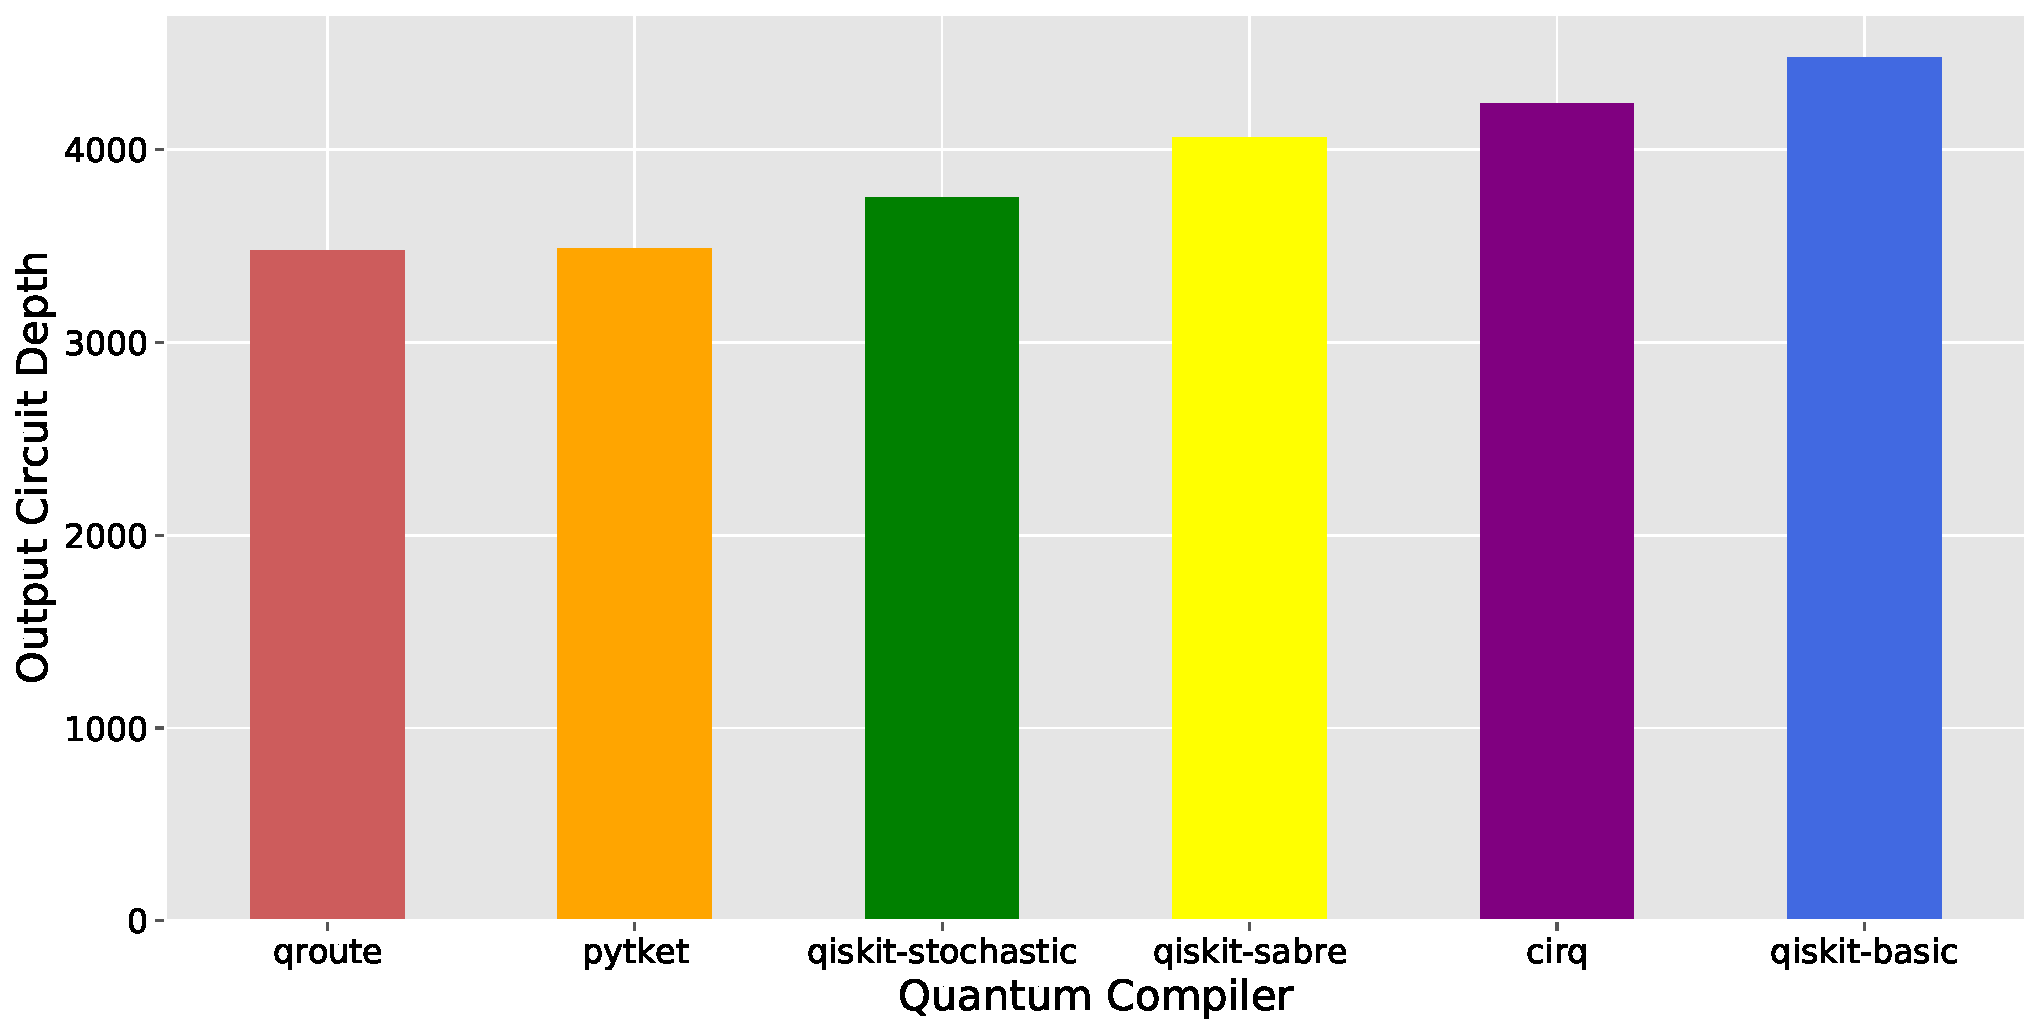
\includegraphics[width=\linewidth]{figures/qroute/sycamore.pdf}
    \caption{\label{fig:supp-sycamore-results}A comparative of the performance of the different routing methods on the small circuit dataset when routing on Google Sycamore device.}
\end{figure}

\onecolumn

\section{Example of Routing Process}

In this section, we show an example run of our algorithm on a $3 \times 3$ device with a normal grid topology, i.e. only qubits adjacent to each other are connected. In the images that follows, we have shown the evolution of the state, the value of the state at each timestep and the action, i.e. the set of gates which are being scheduled. Our MCTS is also responsible for constructing each action by putting together several moves (which are either adding individual gates to the action, or a committing the action for this timestep), that process is not demonstrated in the images. A point to note is that at the start of each timestep, the locks on all qubits may not necessarily be open, because there can be operations which were scheduled in a previous timestep and span over several timesteps. However, this is not the case in our example here where all the gates are assumed to take the same amount of time. We have provided a video simulation of this evolution as a supplementary, as well as the code to visualize this for other circuits.

\begin{figure}[ht]
    \centering
    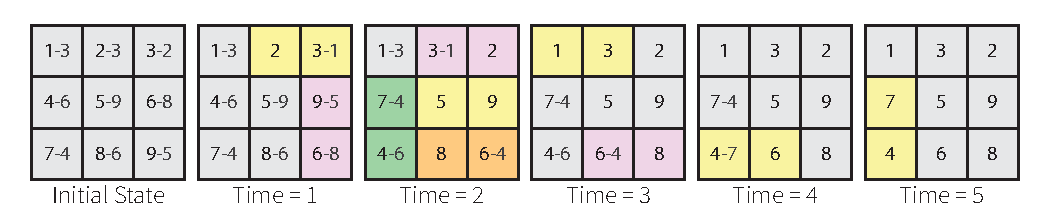
\includegraphics[width=\linewidth]{figures/qroute/Evolution.pdf}
    \caption{\label{fig:supp-evolution}The step by step evolution of the state as the circuit is getting routed. The state is shown on a $3 \times 3$ grid, where in each cell we have the node ID and the next node that it need to participate in a 2-qubit operation with. The yellow and orange colors represent that those 2 qubits have participated in a 2 qubit operation like CNOT, which was scheduled in the previous timestep. The green and purple colors represent that they have just participated in a SWAP operation. Any qubit which is colored was locked in the previous timestep when the action that scheduled it was getting constructed. At time=5, the circuit has been scheduled and none of the qubits have any targets left.}
\end{figure}

\begin{figure}[ht]
    \centering
    \hfill
    \begin{subfigure}[b]{0.38\linewidth}
        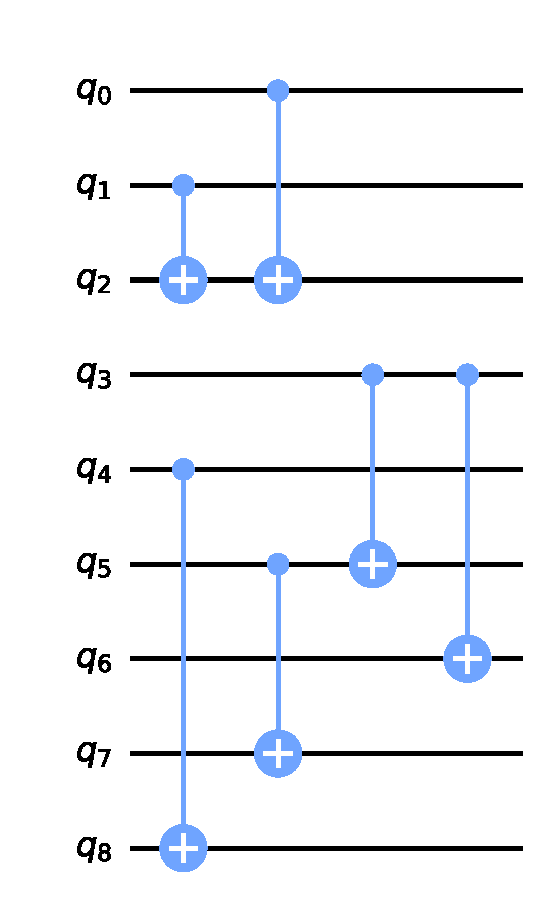
\includegraphics[width=0.7\textwidth]{figures/qroute/supp_circuit_init.pdf}
        \caption{Quantum circuit\label{fig:appendix-orig_circ}}
    \end{subfigure}
    \hfill
    \begin{subfigure}[b]{0.38\linewidth}
        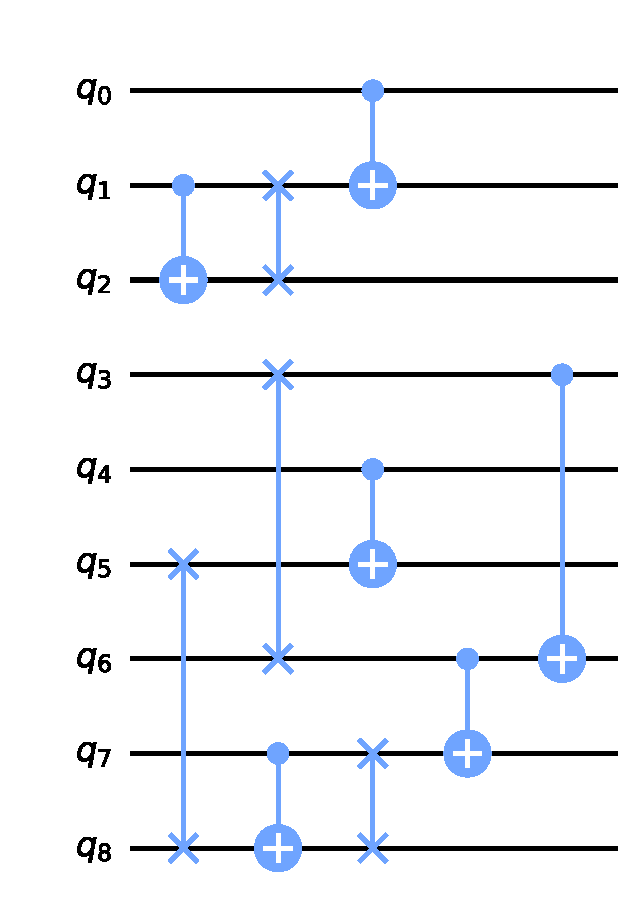
\includegraphics[width=0.82\textwidth]{figures/qroute/supp_circuit_final.pdf}
        \caption{Decomposed circuit\label{fig:appendix-sliced_circ}}
    \end{subfigure}
    \hfill
    \caption{This figure shows the input and output of the routing process shown above in Figure \ref{fig:supp-evolution}. The input circuit was used to decide the targets of the qubits. Gates are added to the output circuit whenever a 2-qubit operation, whether CNOT or SWAP is applied by the router. We can check that both these circuits are equivalent}.
    %Note that the overall unitary operation performed by the circuit is preserved despite the changes in the order of two-qubit gate operations.}
    \label{fig:appendix-routing-example}
\end{figure}

\newpage

\section{Tabulated Results}

\subsection{Random Test Circuits}

\begin{longtable}[c]{|c|c|c|c|c|c|c|c|}
\caption{\textbf{Comparative results for a set of randomly generated test circuits}}
\label{tab:random-circuits}\\
\hline
\multicolumn{2}{|c|}{Input Circuit} & \multicolumn{6}{c|}{Output Circuit Depth} \\ \hline
\# Gates      & \# Layers      & Qroute & Cirq & Qiskit (basic) & Qiskit (stochastic) & Qiskit (sabre) & t$\ket{\text{ket}}$ \\ \hline
\endfirsthead
%
\multicolumn{8}{c}%
{{Table \thetable\ continued from previous page}} \\
\hline
\multicolumn{2}{|c|}{Input Circuit} & \multicolumn{6}{c|}{Output Circuit Depth} \\ \hline
\# Gates      & \# Layers      & Qroute & Cirq & Qiskit (basic) & Qiskit (stochastic) & Qiskit (sabre) & t$\ket{\text{ket}}$ \\ \hline
\endhead
%
30  & 11 & 20 & 29  & 31  & 21  & 24  & 19  \\ \hline
30  & 11 & 19 & 36  & 39  & 23  & 27  & 28  \\ \hline
30  & 10 & 22 & 32  & 28  & 23  & 23  & 23  \\ \hline
30  & 8  & 18 & 24  & 32  & 20  & 33  & 26  \\ \hline
30  & 7  & 17 & 19  & 35  & 17  & 23  & 30  \\ \hline
30  & 11 & 18 & 39  & 34  & 22  & 31  & 26  \\ \hline
30  & 10 & 19 & 22  & 34  & 21  & 20  & 26  \\ \hline
30  & 9  & 17 & 24  & 31  & 21  & 31  & 33  \\ \hline
30  & 10 & 17 & 24  & 36  & 22  & 31  & 21  \\ \hline
30  & 10 & 21 & 23  & 39  & 22  & 27  & 23  \\ \hline
50  & 18 & 31 & 57  & 66  & 41  & 50  & 46  \\ \hline
50  & 17 & 29 & 54  & 63  & 37  & 48  & 46  \\ \hline
50  & 12 & 34 & 47  & 62  & 31  & 50  & 53  \\ \hline
50  & 17 & 28 & 62  & 67  & 38  & 38  & 58  \\ \hline
50  & 17 & 33 & 42  & 61  & 39  & 50  & 51  \\ \hline
50  & 15 & 40 & 49  & 61  & 38  & 48  & 41  \\ \hline
50  & 18 & 35 & 60  & 66  & 38  & 52  & 50  \\ \hline
50  & 18 & 33 & 54  & 53  & 35  & 42  & 52  \\ \hline
50  & 13 & 32 & 58  & 63  & 31  & 39  & 35  \\ \hline
50  & 16 & 30 & 52  & 59  & 37  & 44  & 42  \\ \hline
70  & 19 & 39 & 85  & 93  & 45  & 59  & 76  \\ \hline
70  & 21 & 47 & 96  & 71  & 41  & 56  & 60  \\ \hline
70  & 18 & 46 & 64  & 81  & 43  & 57  & 67  \\ \hline
70  & 21 & 59 & 83  & 84  & 53  & 58  & 79  \\ \hline
70  & 18 & 47 & 67  & 60  & 44  & 55  & 80  \\ \hline
70  & 21 & 45 & 77  & 83  & 46  & 69  & 59  \\ \hline
70  & 19 & 41 & 63  & 76  & 44  & 52  & 74  \\ \hline
70  & 17 & 40 & 68  & 67  & 42  & 62  & 63  \\ \hline
70  & 23 & 37 & 70  & 84  & 52  & 63  & 72  \\ \hline
70  & 23 & 40 & 64  & 91  & 49  & 73  & 60  \\ \hline
90  & 29 & 53 & 106 & 93  & 64  & 80  & 114 \\ \hline
90  & 26 & 64 & 103 & 117 & 64  & 73  & 77  \\ \hline
90  & 28 & 56 & 93  & 111 & 64  & 85  & 89  \\ \hline
90  & 22 & 57 & 94  & 114 & 54  & 75  & 87  \\ \hline
90  & 32 & 58 & 99  & 108 & 66  & 87  & 84  \\ \hline
90  & 23 & 54 & 104 & 127 & 60  & 97  & 90  \\ \hline
90  & 28 & 52 & 96  & 103 & 60  & 80  & 92  \\ \hline
90  & 25 & 50 & 97  & 113 & 60  & 76  & 75  \\ \hline
90  & 23 & 51 & 103 & 107 & 54  & 74  & 82  \\ \hline
90  & 25 & 56 & 96  & 111 & 61  & 79  & 91  \\ \hline
110 & 34 & 63 & 133 & 113 & 72  & 97  & 137 \\ \hline
110 & 27 & 65 & 128 & 143 & 70  & 95  & 118 \\ \hline
110 & 31 & 64 & 117 & 128 & 69  & 95  & 126 \\ \hline
110 & 30 & 73 & 116 & 139 & 66  & 104 & 106 \\ \hline
110 & 32 & 62 & 108 & 129 & 75  & 100 & 124 \\ \hline
110 & 36 & 68 & 112 & 135 & 78  & 93  & 107 \\ \hline
110 & 33 & 94 & 135 & 158 & 74  & 99  & 103 \\ \hline
110 & 33 & 67 & 124 & 110 & 75  & 96  & 117 \\ \hline
110 & 31 & 64 & 114 & 129 & 71  & 101 & 113 \\ \hline
110 & 30 & 65 & 116 & 145 & 69  & 97  & 115 \\ \hline
130 & 33 & 74 & 151 & 149 & 74  & 113 & 154 \\ \hline
130 & 33 & 91 & 135 & 166 & 79  & 122 & 126 \\ \hline
130 & 38 & 77 & 130 & 162 & 91  & 123 & 133 \\ \hline
130 & 32 & 77 & 112 & 153 & 75  & 116 & 139 \\ \hline
130 & 38 & 71 & 145 & 151 & 94  & 113 & 137 \\ \hline
130 & 34 & 66 & 127 & 153 & 79  & 98  & 122 \\ \hline
130 & 35 & 75 & 131 & 151 & 89  & 101 & 144 \\ \hline
130 & 31 & 70 & 114 & 157 & 74  & 107 & 135 \\ \hline
130 & 33 & 76 & 130 & 141 & 79  & 102 & 128 \\ \hline
130 & 41 & 95 & 148 & 161 & 91  & 102 & 114 \\ \hline
150 & 35 & 87 & 175 & 151 & 86  & 109 & 142 \\ \hline
150 & 44 & 92 & 194 & 195 & 104 & 154 & 158 \\ \hline
150 & 38 & 84 & 162 & 177 & 93  & 136 & 149 \\ \hline
150 & 35 & 79 & 128 & 178 & 84  & 123 & 149 \\ \hline
150 & 48 & 96 & 177 & 195 & 101 & 138 & 158 \\ \hline
150 & 43 & 92 & 179 & 167 & 97  & 126 & 142 \\ \hline
150 & 41 & 90 & 171 & 185 & 98  & 120 & 165 \\ \hline
150 & 39 & 85 & 155 & 158 & 91  & 125 & 158 \\ \hline
150 & 39 & 88 & 148 & 182 & 94  & 135 & 158 \\ \hline
150 & 38 & 89 & 178 & 162 & 96  & 123 & 159 \\ \hline
\end{longtable}

\subsection{Small Realistic Circuits}

\begin{longtable}[c]{|c|c|c|c|c|c|c|c|c|}
\caption{\textbf{Comparative results for low-depth realistic test circuits}}
\label{tab:realistic-short-circuits}\\
\hline
\multicolumn{2}{|c|}{Input Circuit} & \multicolumn{7}{c|}{Output Circuit Depth} \\ \hline
Circuit Name & Layers & DQN & Qroute & Cirq & Qiskit & Qiskit & Qiskit & t$\ket{\text{ket}}$ \\
 &  & (Estimate) &  &  & (basic) & (stochastic) & (sabre) &  \\ \hline
\endfirsthead
%
\multicolumn{9}{c}%
{{Table \thetable\ continued from previous page}} \\
\hline
\multicolumn{2}{|c|}{Input Circuit} & \multicolumn{7}{c|}{Output Circuit Depth} \\ \hline
Circuit Name & Layers & DQN & Qroute & Cirq & Qiskit & Qiskit & Qiskit & t$\ket{\text{ket}}$ \\
 &  & (Estimate) &  &  & (basic) & (stochastic) & (sabre) &  \\ \hline
\endhead
%
4gt11\_83 & 14 & 17 & 16 & 22 & 18 & 19 & 18 & 15 \\ \hline
decod24-v0\_38 & 23 & 28 & 30 & 43 & 23 & 31 & 32 & 24 \\ \hline
alu-v3\_34 & 23 & 28 & 27 & 39 & 28 & 28 & 25 & 28 \\ \hline
decod24-v3\_45 & 57 & 68 & 72 & 79 & 74 & 84 & 81 & 77 \\ \hline
4gt4-v0\_80 & 71 & 85 & 89 & 108 & 111 & 91 & 109 & 128 \\ \hline
alu-v0\_27 & 15 & 18 & 16 & 19 & 21 & 19 & 17 & 17 \\ \hline
miller\_11 & 23 & 28 & 25 & 23 & 36 & 36 & 34 & 35 \\ \hline
4gt11\_82 & 18 & 22 & 19 & 28 & 22 & 24 & 23 & 24 \\ \hline
mod10\_176 & 70 & 84 & 83 & 113 & 87 & 94 & 87 & 96 \\ \hline
ex1\_226 & 5 & 6 & 7 & 8 & 10 & 7 & 8 & 6 \\ \hline
4gt5\_75 & 33 & 40 & 38 & 54 & 40 & 41 & 46 & 43 \\ \hline
ising\_model\_10 & 20 & 24 & 23 & 40 & 20 & 20 & 20 & 5 \\ \hline
4gt11\_84 & 8 & 10 & 8 & 13 & 11 & 11 & 12 & 8 \\ \hline
4mod5-v0\_18 & 31 & 37 & 34 & 53 & 39 & 40 & 40 & 33 \\ \hline
alu-v4\_37 & 16 & 20 & 20 & 16 & 23 & 22 & 25 & 24 \\ \hline
qft\_10 & 34 & 41 & 53 & 81 & 113 & 50 & 75 & 49 \\ \hline
4mod5-v0\_19 & 15 & 18 & 17 & 25 & 20 & 19 & 24 & 26 \\ \hline
alu-v0\_27\_example & 15 & 18 & 16 & 18 & 21 & 20 & 17 & 17 \\ \hline
ex-1\_166 & 9 & 11 & 13 & 12 & 14 & 12 & 11 & 13 \\ \hline
4mod7-v1\_96 & 65 & 78 & 75 & 91 & 83 & 97 & 85 & 88 \\ \hline
4mod5-v1\_22 & 10 & 12 & 12 & 17 & 13 & 12 & 12 & 14 \\ \hline
4gt12-v1\_89 & 88 & 105 & 109 & 163 & 126 & 135 & 134 & 125 \\ \hline
alu-v1\_29 & 15 & 18 & 16 & 21 & 19 & 20 & 21 & 19 \\ \hline
mod5d2\_64 & 25 & 30 & 30 & 45 & 30 & 38 & 34 & 31 \\ \hline
4mod7-v0\_94 & 66 & 79 & 77 & 131 & 83 & 92 & 92 & 82 \\ \hline
4gt13\_91 & 46 & 55 & 53 & 64 & 52 & 68 & 60 & 52 \\ \hline
4mod5-v0\_20 & 9 & 11 & 11 & 16 & 17 & 10 & 10 & 10 \\ \hline
alu-v2\_33 & 15 & 18 & 19 & 26 & 17 & 19 & 20 & 17 \\ \hline
4\_49\_16 & 91 & 109 & 99 & 138 & 107 & 129 & 104 & 128 \\ \hline
decod24-v2\_43 & 22 & 27 & 25 & 38 & 26 & 28 & 33 & 25 \\ \hline
4gt10-v1\_81 & 60 & 72 & 71 & 113 & 82 & 80 & 81 & 75 \\ \hline
alu-bdd\_288 & 35 & 42 & 47 & 60 & 55 & 52 & 54 & 44 \\ \hline
4mod5-v1\_23 & 30 & 36 & 33 & 46 & 45 & 45 & 48 & 40 \\ \hline
one-two-three-v2\_100 & 29 & 35 & 35 & 40 & 41 & 41 & 40 & 39 \\ \hline
rd53\_138 & 42 & 50 & 54 & 70 & 67 & 69 & 78 & 59 \\ \hline
alu-v2\_32 & 64 & 77 & 72 & 96 & 88 & 87 & 98 & 96 \\ \hline
rd32\_270 & 35 & 42 & 38 & 53 & 48 & 53 & 49 & 40 \\ \hline
aj-e11\_165 & 63 & 75 & 73 & 103 & 82 & 90 & 81 & 82 \\ \hline
4gt12-v0\_88 & 77 & 92 & 90 & 128 & 116 & 111 & 107 & 140 \\ \hline
decod24-v1\_41 & 35 & 42 & 38 & 55 & 42 & 50 & 47 & 43 \\ \hline
3\_17\_13 & 17 & 21 & 24 & 17 & 26 & 18 & 24 & 22 \\ \hline
4mod5-v0\_19 & 16 & 20 & 17 & 27 & 16 & 21 & 22 & 13 \\ \hline
mini\_alu\_305 & 53 & 64 & 63 & 113 & 86 & 81 & 79 & 81 \\ \hline
one-two-three-v0\_98 & 59 & 71 & 71 & 82 & 69 & 81 & 77 & 87 \\ \hline
4gt13\_90 & 50 & 60 & 54 & 72 & 56 & 63 & 56 & 80 \\ \hline
4mod5-bdd\_287 & 31 & 37 & 41 & 48 & 35 & 48 & 50 & 35 \\ \hline
ham3\_102 & 11 & 14 & 14 & 16 & 15 & 16 & 15 & 9 \\ \hline
alu-v1\_28 & 16 & 20 & 16 & 21 & 20 & 18 & 22 & 18 \\ \hline
rd32-v0\_66 & 16 & 20 & 19 & 20 & 20 & 20 & 20 & 14 \\ \hline
cnt3-5\_179 & 43 & 52 & 64 & 91 & 72 & 61 & 65 & 83 \\ \hline
4gt13\_92 & 26 & 31 & 30 & 41 & 33 & 38 & 36 & 29 \\ \hline
alu-v4\_36 & 47 & 56 & 55 & 59 & 65 & 68 & 61 & 60 \\ \hline
rd32-v1\_68 & 16 & 20 & 17 & 21 & 20 & 20 & 20 & 14 \\ \hline
4gt13-v1\_93 & 27 & 33 & 29 & 34 & 35 & 36 & 36 & 31 \\ \hline
4gt5\_76 & 42 & 50 & 47 & 69 & 53 & 52 & 53 & 53 \\ \hline
mod5d1\_63 & 11 & 14 & 14 & 17 & 12 & 12 & 14 & 14 \\ \hline
graycode6\_47 & 5 & 6 & 5 & 9 & 5 & 5 & 5 & 5 \\ \hline
xor5\_254 & 5 & 6 & 5 & 8 & 10 & 8 & 8 & 6 \\ \hline
decod24-bdd\_294 & 31 & 37 & 34 & 50 & 40 & 40 & 46 & 37 \\ \hline
alu-v0\_26 & 35 & 42 & 41 & 62 & 47 & 48 & 45 & 54 \\ \hline
mod5mils\_65 & 16 & 20 & 19 & 21 & 17 & 21 & 25 & 18 \\ \hline
alu-v3\_35 & 16 & 20 & 20 & 25 & 23 & 21 & 21 & 24 \\ \hline
one-two-three-v1\_99 & 56 & 67 & 60 & 87 & 70 & 84 & 70 & 95 \\ \hline
one-two-three-v3\_101 & 29 & 35 & 34 & 43 & 36 & 37 & 38 & 46 \\ \hline
4gt5\_77 & 51 & 61 & 61 & 78 & 63 & 66 & 70 & 66 \\ \hline
\end{longtable}

\subsection{Large Realistic Circuits}
\begin{longtable}[c]{|c|c|c|c|c|c|c|}
\caption{\textbf{Comparative results for long-depth realistic test circuits}}
\label{tab:realistic-large-circuits}\\
\hline
\multicolumn{2}{|c|}{Input Circuit} & \multicolumn{5}{c|}{Output Circuit Depth} \\ \hline
\endfirsthead
%
\multicolumn{7}{c}%
{{Table \thetable\ continued from previous page}} \\
\hline
\multicolumn{2}{|c|}{Input Circuit} & \multicolumn{5}{c|}{Output Circuit Depth} \\ \hline
\endhead
%
Circuit Name & Number of Gates & Qroute & t$\ket{\text{ket}}$ & Qiskit (basic) & Qiskit (stochastic) & Qiskit (sabre) \\ \hline
rd84\_142 & 154 & 120 & 154 & 142 & 138 & 133 \\ \hline
adr4\_197 & 1498 & 1580 & 1770 & 1840 & 1968 & 1988 \\ \hline
radd\_250 & 1405 & 1504 & 1799 & 1812 & 1815 & 1888 \\ \hline
z4\_268 & 1343 & 1400 & 1670 & 1623 & 1718 & 1914 \\ \hline
sym6\_145 & 1701 & 1806 & 2167 & 2168 & 2261 & 2299 \\ \hline
misex1\_241 & 2100 & 2231 & 2580 & 2770 & 2681 & 2944 \\ \hline
rd73\_252 & 2319 & 2468 & 2793 & 2943 & 3071 & 3132 \\ \hline
cycle10\_2\_110 & 2648 & 2941 & 3380 & 3418 & 3485 & 3705 \\ \hline
square\_root\_7 & 3089 & 3327 & 4560 & 3759 & 3822 & 3695 \\ \hline
sqn\_258 & 4459 & 4779 & 5535 & 5526 & 5696 & 6252 \\ \hline
rd84\_253 & 5960 & 6264 & 7507 & 7411 & 7537 & 8843 \\ \hline
\end{longtable}